%!TEX program = xelatex
% 完整编译: xelatex -> bibtex -> xelatex -> xelatex
\documentclass[lang=cn,11pt,a4paper,cite=numbers]{elegantpaper}

\title{Simultaneuous Multi-Slice(SMS) pMRI}
%\institute{\href{https://elegantlatex.org/}{Elegant\LaTeX{} 项目组}}
\date{\zhtoday}
% 本文档命令
\usepackage{array}
\usepackage{graphicx}
\newcommand{\ccr}[1]{\makecell{{\color{#1}\rule{1cm}{1cm}}}}
\begin{document}

\maketitle

\section{SMS-pMRI model}
\par 假设$u_1, u_2,\dots, u_S$是需要被重建的未知切片图像,$S$表示切片数量,使用$y$表示采集得到的$k$-space数据,其维度大小为row $\times$ column $\times$ L $\times$ S,其中row和column分别是图像长和宽,L表示$k$-space数据中的线圈数量,S表示切片数量,则SMS-pMRI模型可以写成:
\begin{equation}
	PF_{3D}Cu = y
\end{equation}
其中$y$是$k$-space数据的向量化形式,$y=(y_1,y_2,\dots,y_S)^T,y_s=(y_s^{1},y_s^{2}, \dots,y_s^{L})^T$, 即$y_s^{L}$表示第$s$个切片中第$L$个线圈数据。$u=(u_1,u_2,\dots, u_s)^T$,其中$u_i,i=1,\dots,s$表示第$i$个切片图像的向量化形式。$C$是线圈灵敏度矩阵,$Cu$具体为:
\begin{equation}
	Cu \leftrightarrow
	\begin{bmatrix}
		f(u_1c_1) \\
		\vdots \\
		f(u_Sc_S)\\
	\end{bmatrix},
	\quad
	f(u_i c_i) \leftrightarrow
	\begin{bmatrix}
		u_i \otimes c_i^{1} \\
		\vdots \\
		u_i \otimes c_i^{L}\\
	\end{bmatrix}	
\end{equation}
$F_{3D}$表示3D快速傅里叶变换,该操作将数据reshape成大小为row $\times$ column $\times$ S $\times$ L,然后沿着线圈方向进行傅里叶变换,变换后再reshape成大小为row $\times$ column $\times$ L $\times$ S,最近进行向量化操作。如图1所示,此时已经将向量化的数据进行大小变换,即将不同Slice之间同一线圈的数据进行堆叠,并且对同一个线圈的数据进行3D傅里叶变换。$P$表示采样矩阵,定义为
\begin{equation}
	P=
	\begin{bmatrix}
		P_1 & & 0\\
		& \ddots& \\
		0& & P_S
	\end{bmatrix}
\end{equation}
% TODO: \usepackage{graphicx} required
\begin{figure}
	\centering
	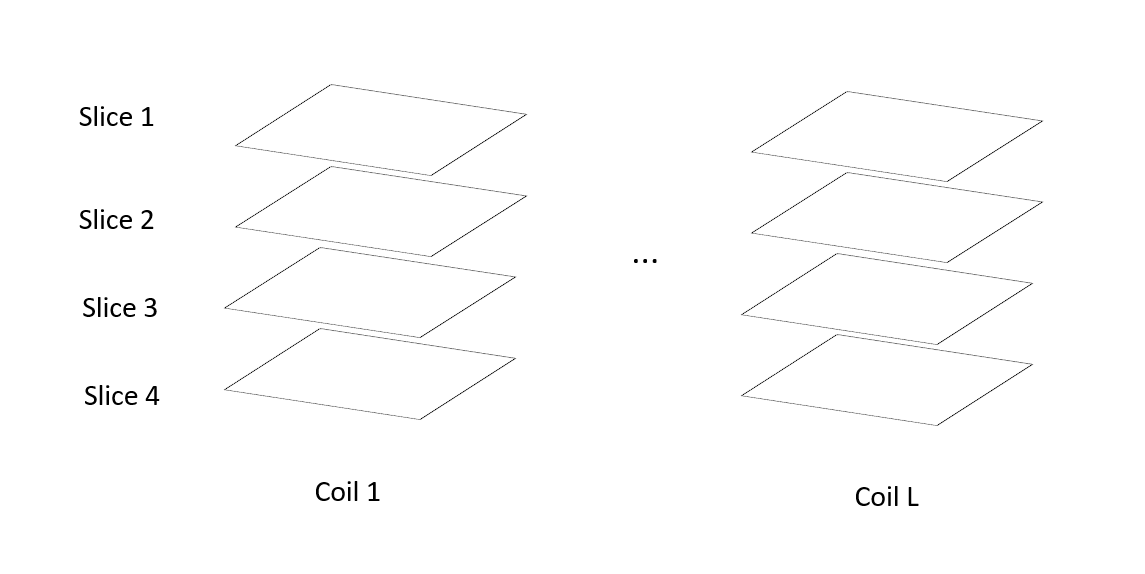
\includegraphics[width=0.7\linewidth]{screenshot001}
	\caption{进行3D傅里叶变换时的数据形式}
	\label{fig:screenshot001}
\end{figure}


\section{Optimization model for SENSE reconstruction}
\par 模型(1)是一个高度欠定的方程,因此可以采用带有正则化的最小二乘法进行求解,求解模型可以定义为
\begin{equation}
	\hat{u} = argmin \left\lbrace \frac{1}{2} \Vert PF_{3D}Cu - y \Vert_2^2 + \lambda \Vert W_{3D}u \Vert_1 \right\rbrace 
\end{equation}
令 $K=PF_{3D}C, f(u) = \frac{1}{2} \Vert Ku - y \Vert_2^2,h(u)=\lambda \Vert W_{3D}u \Vert_1 $,模型(4)可以使用PD3O算法进行求解,求解流程为
\begin{equation}
	\left\{
	\begin{aligned}
		s^{k+1} &= prox_{\delta h^{*}}((I-\gamma \delta WW^T)s^k + \delta W(u^k -\gamma \nabla f(u^k))) \\
		u^{k+} &=u^k-\gamma \nabla f(u^k) - \gamma W^T s^{k+1}
	\end{aligned}
	\right.
\end{equation}

\section{Experiments}
\par uniform采样,采样率为41,ACS=41,每个Slice使用相同的采样矩阵,$\lambda = 0.0000001$, 重建图如图2所示。
% TODO: \usepackage{graphicx} required
% TODO: \usepackage{graphicx} required
\begin{figure}
	\centering
	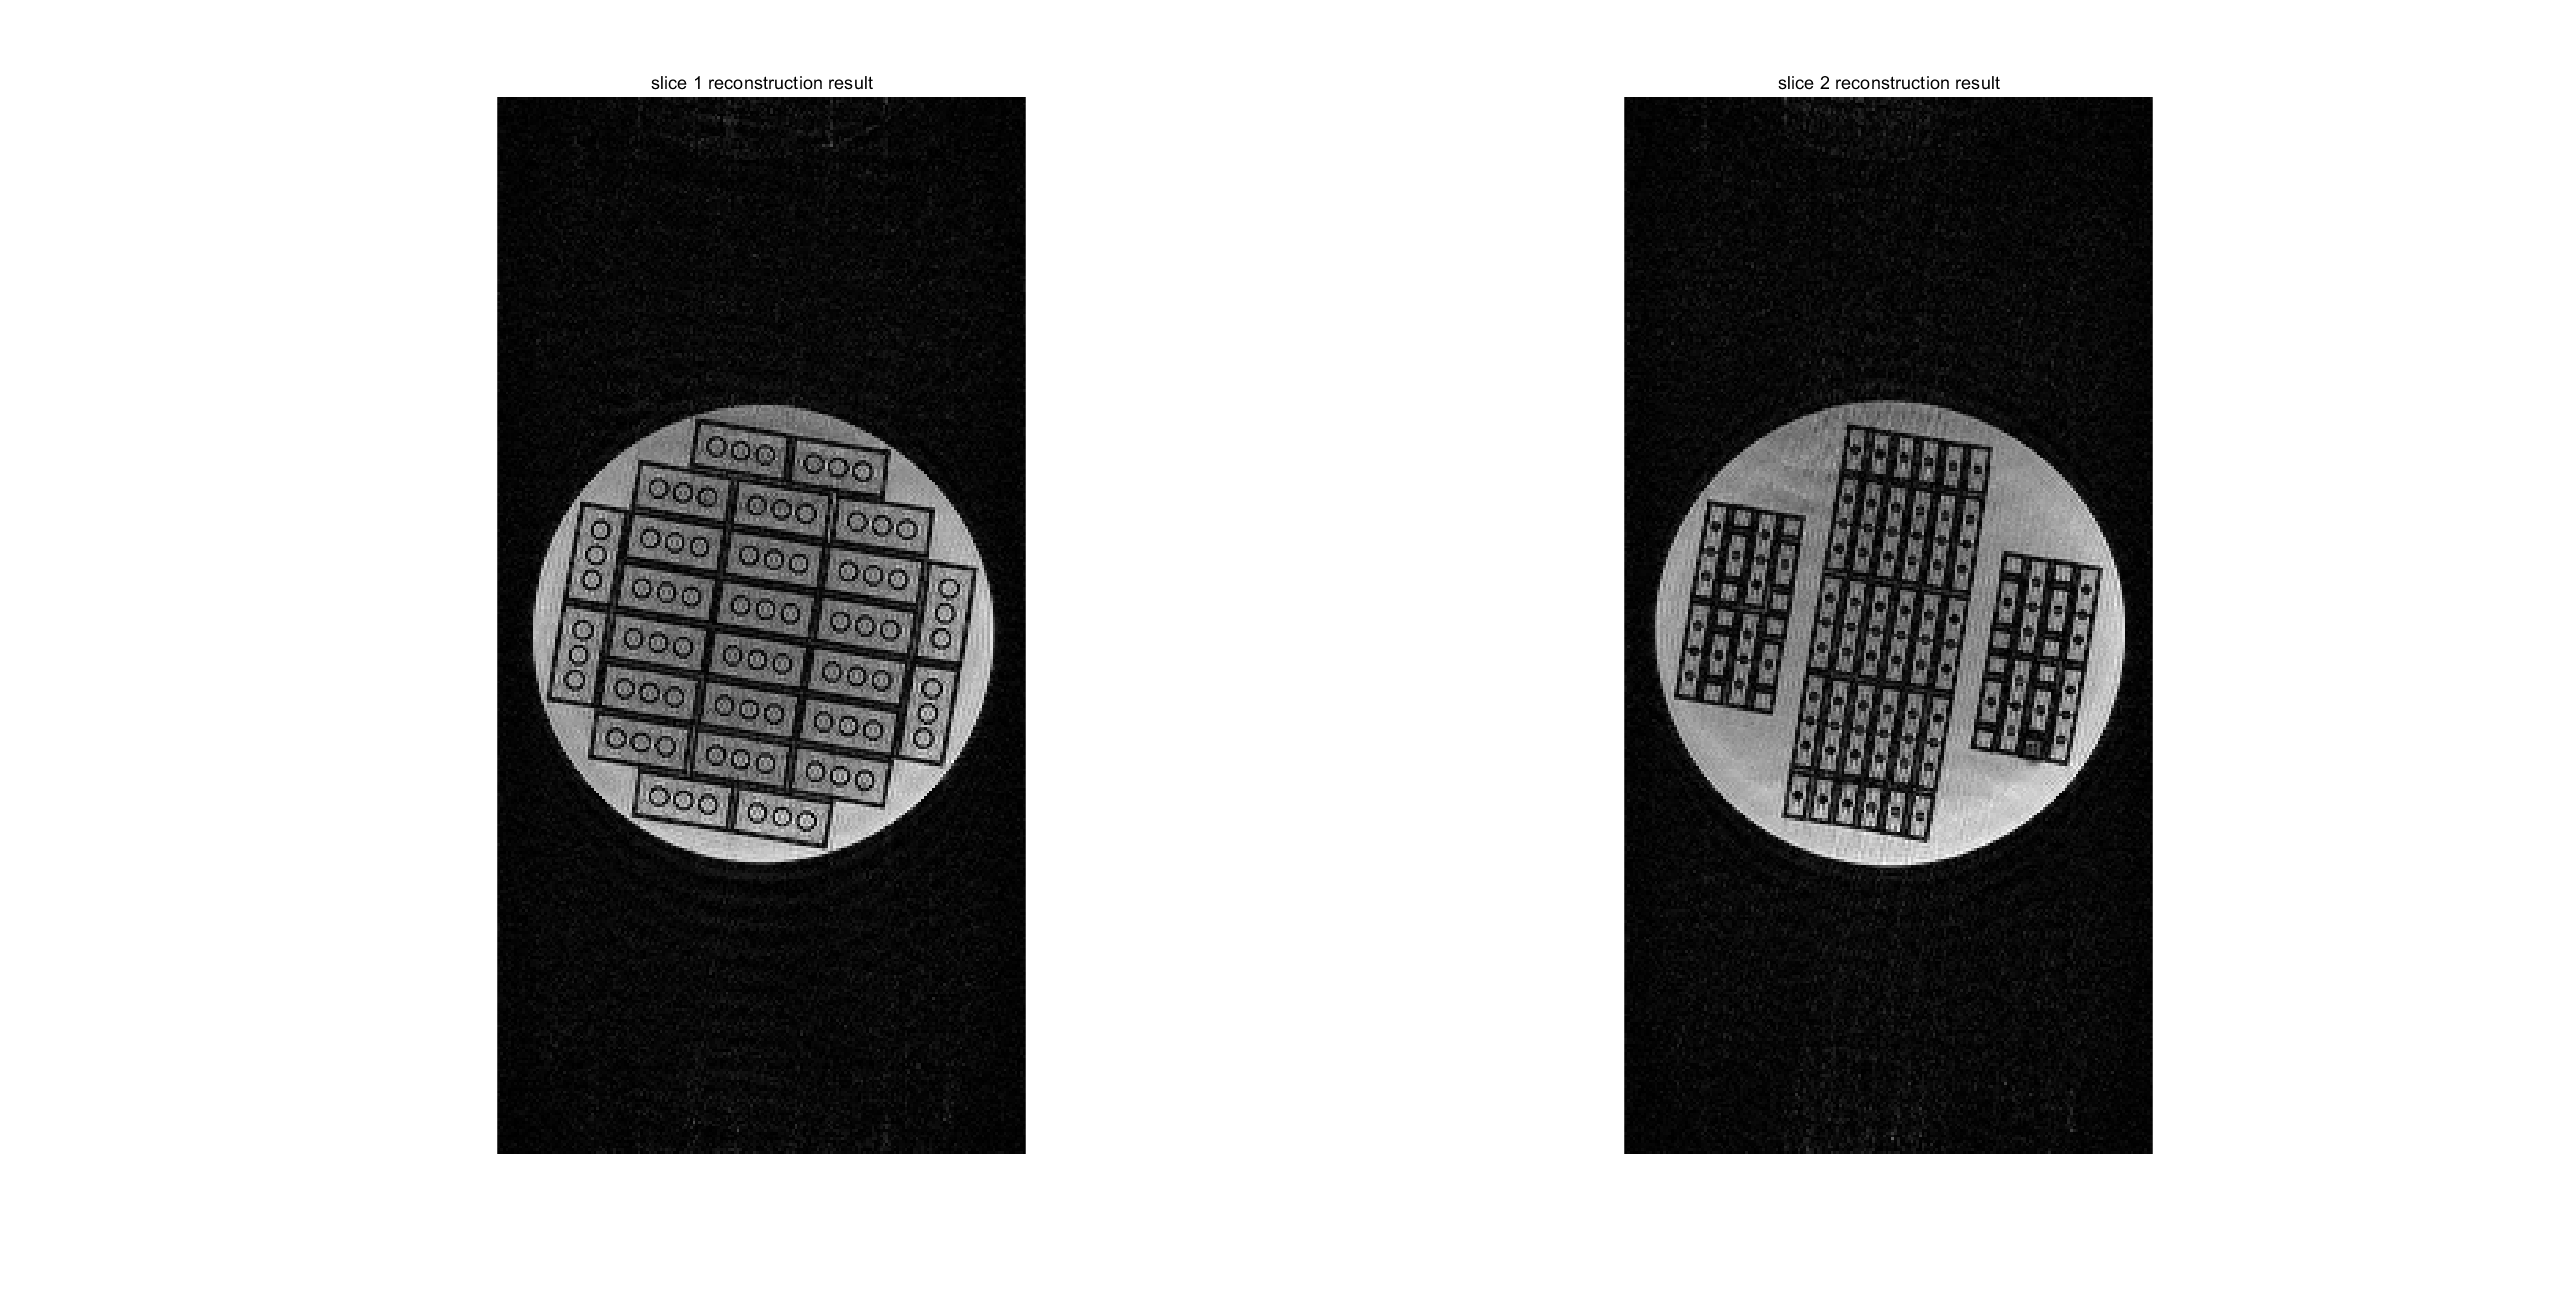
\includegraphics[width=0.7\linewidth]{rec}
	\caption{重建图}
	\label{fig:rec}
\end{figure}

% TODO: \usepackage{graphicx} required
\begin{figure}
	\centering
	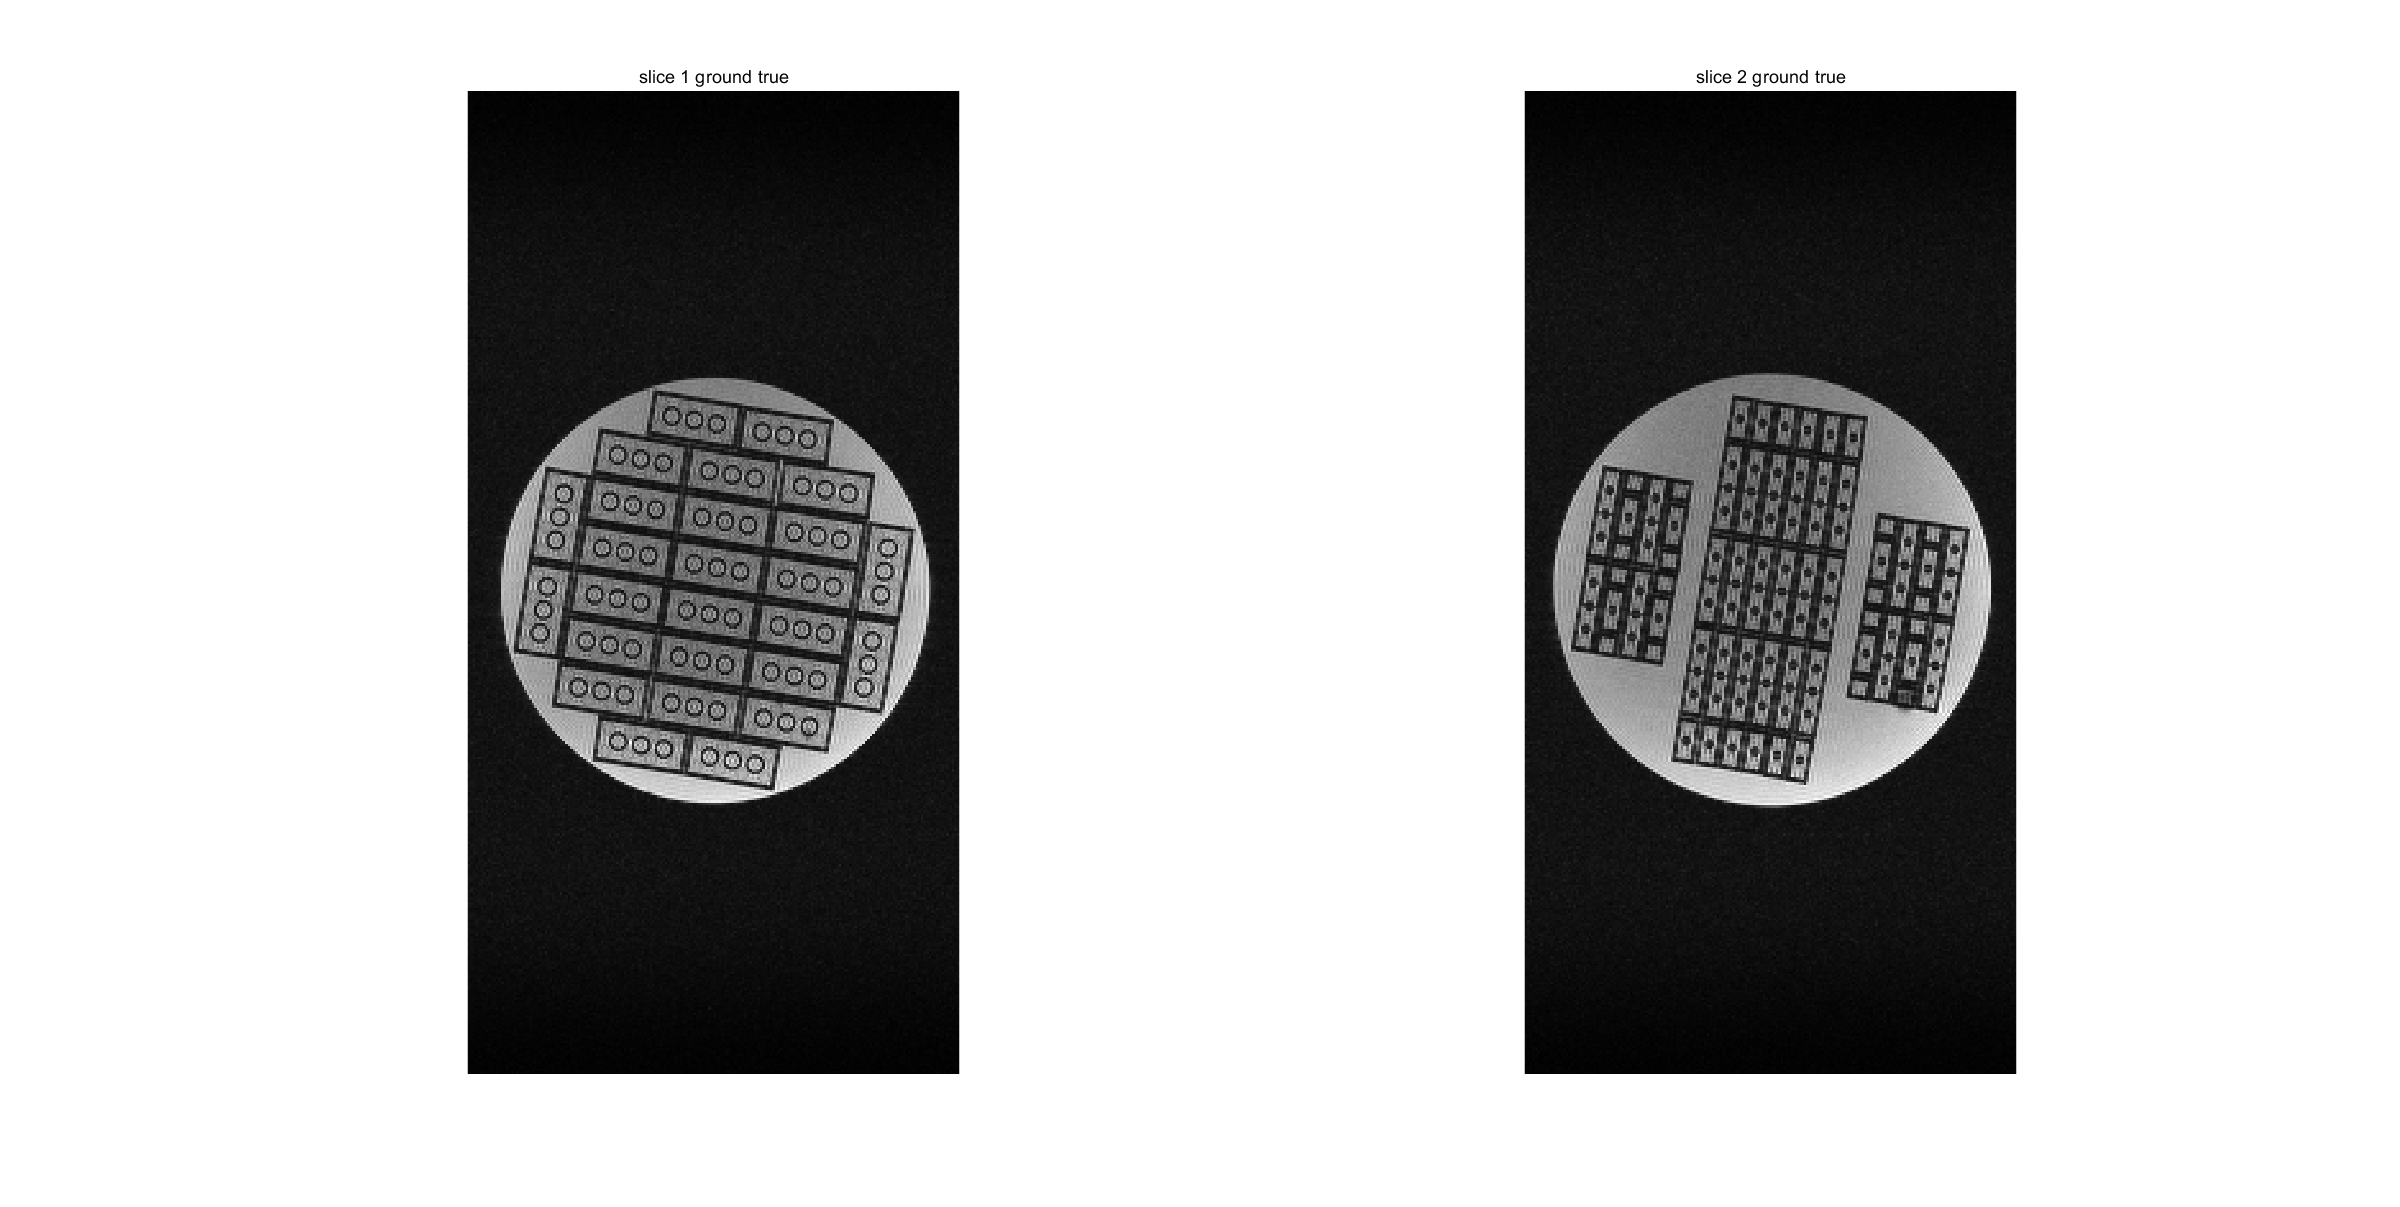
\includegraphics[width=0.7\linewidth]{true}
	\caption{参考图像}
	\label{fig:true}
\end{figure}



\end{document}
